\section{Finding 2: Non-transferable Null Models}
\label{sec:f2}

\subsection{Cross-domain calibration is a net negative}
Empirical thresholds are fitted on a null corpus; the implicit assumption is
that the null distribution \emph{transfers}. We measure it across six text
domains: in-domain technical prose (control), English literature (Gutenberg),
classical Chinese novels (Hongloumeng), code-comment text, short fragments
(800 chars, the documented weak band), and repetitive templates. Each domain
is tested under three configurations: uncalibrated defaults; calibration on
the technical-prose corpus (cross-domain); and calibration on the first half
of the same domain (in-domain). Metrics: existence FPR and attribution FPR
on 100 null texts with a 50-user registry (25--56 texts where the corpus
allows), plus a TPR control on the same texts watermarked and traced with
metadata.

\begin{table}[t]
\centering\small
\caption{E-B3: existence FPR / attribution FPR / TPR by domain and
calibration configuration (zero-cost codec, explicit-salt path; $n$ per
domain). Cross-domain calibration degrades FPR below the uncalibrated
baseline everywhere; in-domain calibration restores it except when the
calibration corpus is too small (demo, $n{=}14$).}
\label{tab:eb3}
\begin{tabular}{@{}l@{\hspace{4pt}}c@{\hspace{4pt}}ccc@{}}
\toprule
Domain ($n$) &  & Uncalibrated & Cross-domain & In-domain \\
\midrule
demo control (29) & FPR & 0.069 & 0.035 & \textbf{0.467} \\
& attr & 0.000 & 0.000 & 0.000 \\
& TPR & 0.483 & 1.000 & 1.000 \\
\midrule
English lit.\ (100) & FPR & 0.000 & 0.430 & 0.060 \\
& attr & 0.000 & 0.000 & 0.000 \\
& TPR & 0.040 & 0.950 & 0.740 \\
\midrule
Chinese lit.\ (100) & FPR & 0.030 & 0.550 & 0.000 \\
& attr & 0.010 & 0.010 & 0.000 \\
& TPR & 0.620 & 0.980 & 0.980 \\
\midrule
code comment (25) & FPR & 0.000 & 0.080 & 0.077 \\
& attr & 0.000 & 0.000 & 0.000 \\
& TPR & 0.120 & 1.000 & 1.000 \\
\midrule
short fragments (56) & FPR & 0.018 & 0.089 & 0.036 \\
& attr & 0.000 & 0.000 & 0.000 \\
& TPR & 0.089 & 0.929 & 0.964 \\
\midrule
template (100) & FPR & 0.680 & 0.840 & 0.020 \\
& attr & 0.210 & 0.110 & 0.000 \\
& TPR & 1.000 & 1.000 & 1.000 \\
\bottomrule
\end{tabular}
\end{table}

Table~\ref{tab:eb3} gives the full matrix. Three regularities stand out.
First, \emph{cross-domain calibration is a net negative}: FPR rises from
0--6.9\% (uncalibrated) to 3.5--84\% in every domain---the calibrated
verifier is worse than the naive one. The zero distribution of $z$-scores is
governed by vocabulary habits; what counts as ``normal fluctuation'' in
technical prose is not normal in classical fiction. Second, \emph{in-domain
calibration works but has a size floor}: FPR returns to 0--7.7\% except in
the demo control, where only 14 calibration documents were available and
FPR stays at 46.7\%. Corpus size matters as much as domain match; we
recommend $\ge$20 documents as a minimum and $\ge$50 for production.
Third, uncalibrated defaults are conservative (FPR $\approx$ 0) but TPR
collapses out of domain (4\% on English literature, 9\% on short
fragments): calibration is not optional, it must simply be in-domain.

\begin{figure}[t]
\centering
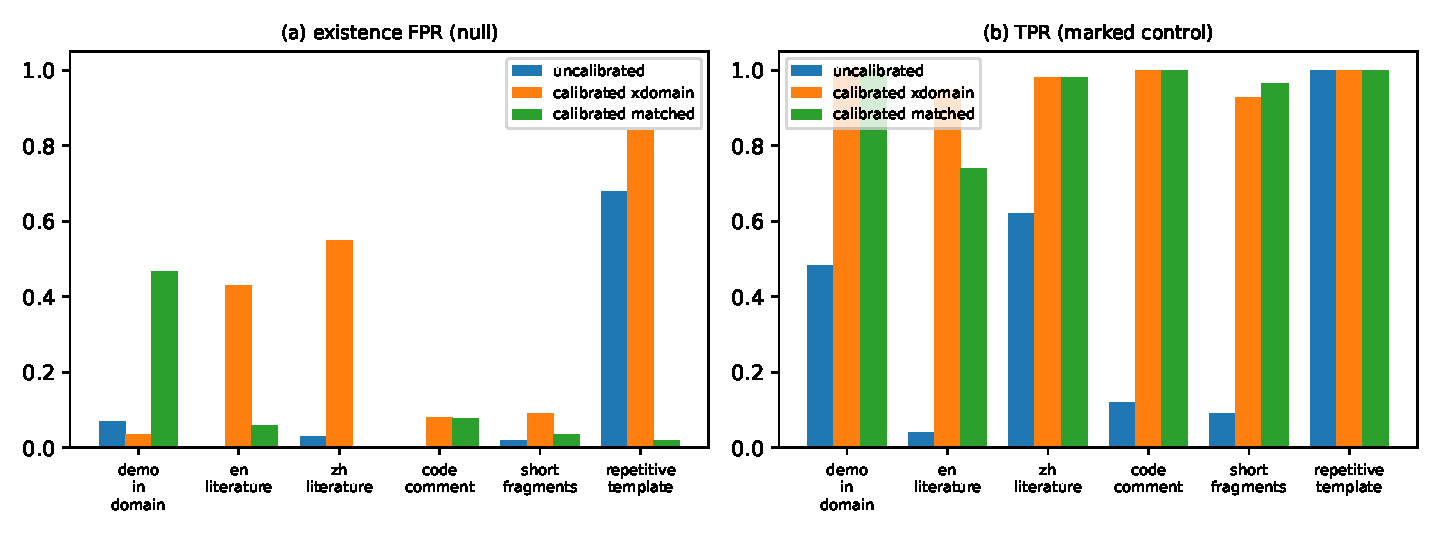
\includegraphics[width=\columnwidth]{figures/fig_eb3_domain_matrix.pdf}
\caption{E-B3: (a) existence FPR and (b) TPR across six domains and three
calibration configurations.}
\label{fig:eb3}
\end{figure}

\subsection{Comparison with a presence-ratio statistic}
Is Finding 2 a property of $z$-test statistics in particular? We repeated
the cross-domain measurement on the official PostMark implementation
(EMNLP 2024; presence ratio over a 3266-word embedding-derived list).
Fitting a $q_{99}$ threshold on Gutenberg nulls and testing on C4 web text
yields 5.0\% FPR (reverse direction: 0.5\%); matched controls give 2.0\%
and 0.0\% (nominal 1\%, $n{=}200$ per cell). PostMark's bounded,
per-text-adaptive statistic is measurably more domain-stable than the
$z$-test family---but, as \S\ref{sec:f3} shows, the families also differ on
the template attack. Pitfall severity is \emph{statistic-dependent}; our
deployment checklist (\S\ref{sec:recs}) is written per statistic.
An end-to-end rerun of PostMark's official embedding pipeline in our own
environment (nomic word selection locally; the v2 insertion loop with a
32B API inserter; $n{=}60$ C4 texts) restores the positive control that
the cross-environment artifact mismatch (Appendix) had invalidated:
TPR at 1\% FPR is 1.0, with presence rising from 0.10 (null) to 0.57 (watermarked). The null-side transfer measurements above therefore stand
on a validated detector.
